% !TEX TS-program = pdflatex

\documentclass[unicode,11pt,notheorems,xcolor=table]{beamer}

\usepackage[T2A]{fontenc}
\usepackage[utf8]{inputenc}
\usepackage[russian]{babel}
\usepackage{amsmath,amsfonts,amssymb,amsthm}
\usepackage{mathtools}
\usepackage{diagbox}

\usepackage{ulem}
\usepackage{tikz, graphicx}
%\usepackage{tkz-graph}
\usetikzlibrary{matrix,arrows,decorations.pathmorphing, arrows.meta,positioning}
\usetikzlibrary{positioning,calc}
\usetikzlibrary{petri}
\usetikzlibrary{decorations.pathreplacing}

%Описание стиля презентации
\usetheme[sidebar=0]{kfmn} 
\setbeamercovered{transparent}

%\definecolor{cyan}{RGB}{240,217,1}
%\definecolor{vgugreen}{RGB}{143,188,103}
%\definecolor{vgured}{RGB}{234,38,40}
%\definecolor{vgublue}{RGB}{53,101,167}



\makeatletter
	\g@addto@macro{\endtabular}{\rowfont{}}% Clear row font
	\makeatother
	\newcommand{\rowfonttype}{}% Current row font
	\newcommand{\rowfont}[1]{% Set current row font
		\gdef\rowfonttype{#1}#1\ignorespaces%
	}
\makeatother

\newcommand{\myunit}{9mm}
\tikzset{
    node style sp/.style={draw,circle,minimum size=\myunit},
    node style ge/.style={circle,minimum size=\myunit},
    arrow style mul/.style={draw,sloped,midway,fill=white},
    arrow style plus/.style={midway,sloped,fill=white},
}

%[0, 6, 8, 8, 10, 5, 6, 10, 8, 10, 10], 

\pgfdeclareimage[height=8mm]{university-logo}{logo-iem.png}
\logo{\pgfuseimage{university-logo}}
%2[0, 11, 10, 8, 11, 5, 11, 11, 8, 11, 10, 11],

\titlepicture{
	\begin{tikzpicture}[y=1.4cm,overlay,rotate=8]
	\coordinate (O) at (-3cm,0.9cm);
	\filldraw[thick,draw= vgublue, fill=vgublue!20!white] (0,0) circle[radius=4.2cm];
	\clip (0,0) circle[radius=4.2cm];
	\draw (-1.5,1.5) node{
	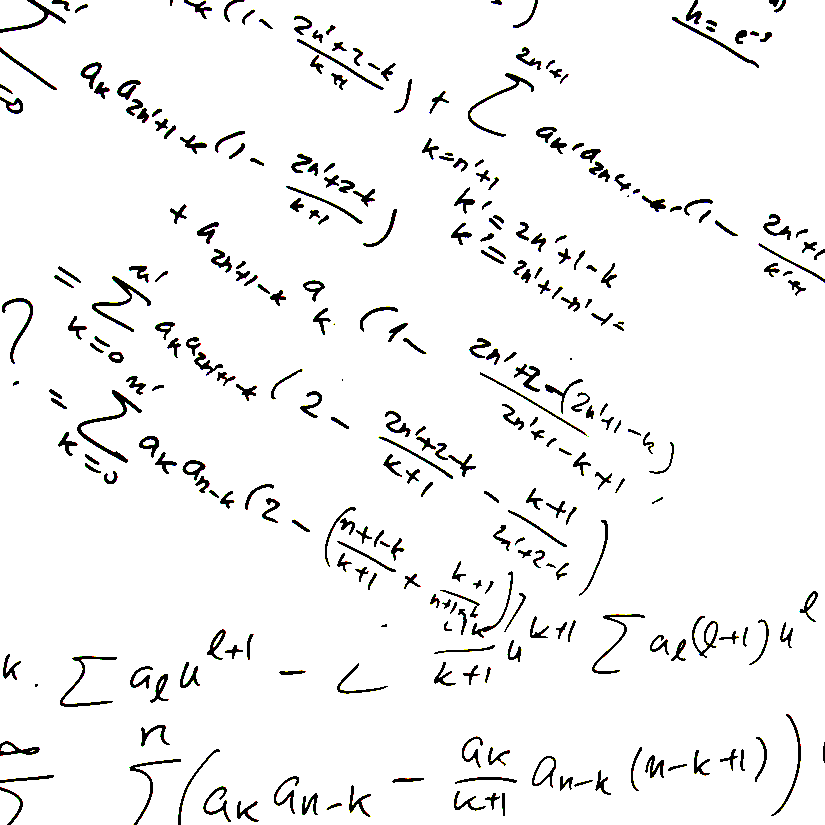
\includegraphics[width=8cm]{titlepic.png}
	};
\end{tikzpicture}
}

\usepackage[math]{iwona}

\newcommand{\hplus}{\mathbin{\hat+}}
\newcommand{\hdot}{\mathbin{\hat\cdot}}
% Описание теорем
\newtheorem{theorem}{Теорема}
\newtheorem{seq}{Следствие}
%%

\LECT % 

% Титульный лист теорем
\author[Д.\,В. Чупраков]{канд.\,физ.-матем.\,наук, доцент Д.\,В. Чупраков\\[6pt] usr10381@vyatsu.ru}

\institute[ВятГУ]{ФГБОУ ВО Вятский государственный университет}

\department{Факультет экономики и финансов}

\title[Лекция~9. Модель управления запасами]{
	Введение в экономико-математическое моделирование\\[12pt]
	Лекция~9. Модель управления запасами}

\date{2 ноября 2020~г.}


\setbeamercovered{invisible}



\begin{document}


\maketitle

\begin{frame}{Структура лекции}
	\tableofcontents
\end{frame}

\section{Основные понятия}

\begin{frame}{Задача управления запасами}
    \begin{block}{Определение}
        Совокупность временно не используемых экономических ресурсов, называют \alert{запасами предприятия}. 
    \end{block}

    \begin{itemize}
        \item сырье, 
        \item основные и вспомогательные материалы, 
        \item парк техники
        \item полуфабрикаты
        \item готовая продукция
    \end{itemize}

    \pause
    \begin{block}{Задача управления заказами}
        Определении объемов поставок и периодичности заказов, при которых издержки (функция затрат) принимают минимальное значение.
    \end{block}
\end{frame}

\begin{frame}{Виды издержек}
    
    Количество товара, поставляемое на склад, называют \alert{размером партии.}
    
    \begin{itemize}
        \item \structure{$L_1$}~--- \alert{организационные издержки}~--- расходы, связанные с оформлением и доставкой товаров;
        \item \structure{$L_2$}~--- \alert{издержки, связанные с приобретением запасов}~--- стоимость партии товаров. 
        \item \structure{$L_3$}~---\alert{издержки содержания запасов}~--- затраты, связанные с хранением, амортизация запасов. 
        \item  \structure{$L_4$}~---\alert{издержки, связанные с дефицитом}~--- денежный штраф, потеря лояльности потребителей.
    \end{itemize}
\end{frame}

% \begin{frame}{Виды спроса}
%     Спрос на предметы потребления может быть 
%     % (см. с. 47, 212 издания [19]):
%     \begin{itemize}
%         \item стационарным или нестационарным;
%         \item детерминированным или стохастическим;
%         \item непрерывно распределенным или дискретным;
%         \item зависящим от спроса на другие товары или независимым.
%     \end{itemize}
% \end{frame}

\begin{frame}{Виды задач управления запасами}
%      Многообразием
% реальных ситуаций вызвана необходимость рассмотрения огромного числа вариантов задач управления запасами. В зависимости
% от числа периодов, на которые планируются операции, различают
\begin{itemize}
    \item статические – рассматривается один период времени;
    \item динамические – рассматривается несколько периодов
    времени
    % (см. с. 21 издания [19]).
\end{itemize}
\end{frame}


\begin{frame}{Пополнение запасов}
    Пополнение запасов, как правило, происходит с некоторой случайной задержкой относительно момента выдачи требования
%  (подробнее см. с. 133 учебного издания [19]):
\begin{itemize}
    \item мгновенная поставка;
    \item задержка поставок на фиксированный срок;
    \item задержка поставок на случайный интервал времени (распределенный по известному вероятностному закону).
\end{itemize}
\end{frame}


\begin{frame}{График изменения запаса}
    
    % Под $Q$ будем понимать количество изделий или материалов
    % (товаров) только одного вида. Если на изделие поступает заявка,
    % то оно отпускается, и значение Q падает. Предположим, что вели-
    % чина спроса непрерывна во времени. Если Q = 0, то имеет место
    % дефицит.
\end{frame}


% \section{Производная и немного школы}

\section{Основная модель управления запасами}
\begin{frame}{}
    \begin{block}{}
        \centering \LARGE \structure{Основная модель управления запасами}
        \par
    \end{block}
    
    Готовые товары поступают на склад партиями
\end{frame}


\begin{frame}{Основная модель управления запасами}
    \alert{Основная модель управления запасами}~--- это 
    модель, удовлетворяющая следующим гипотезам:
    \begin{itemize}
        \item Рассматривается один вид товара
        \item Спрос постоянен и непрерывен; весь спрос удовлетворяется.
        \item Издержки постоянны и не зависят от размера партии.
        \item Цена единицы товара постоянна. 
        \item Стоимость хранения единицы товара в течение периода времени постоянна.
        \item Размер партии постоянен. 
        \item \alert{Поступление товара происходит мгновенно, как только уровень запаса равен нулю.}
\end{itemize}
\end{frame}

\begin{frame}{Основные величины модели ОМУЗ}
\begin{itemize}
    % \item \structure{$V$}~--- спрос \hfill  (ед. товара)
    \item \structure{$v$}~--- интенсивность спроса   \hfill
        (ед. товара за ед. времени)
    \item \structure{$k$}~--- организационные издержки\hfill (ден. ед. за ед. поставки)
    \item  \structure{$s$}~--- стоимость товара  \hfill (ден. ед. за ед. товара)
    \item \structure{$h$}~--- издержки содержания запасов \\\hfill (ден. ед. за ед. товара в ед. времени)
    \item \structure{$q$}~--- размер партии \hfill (ед. товара)
\end{itemize}
\end{frame}
\begin{frame}{График изменения запасов ОМУЗ}{}
    {\centering
    \begin{tikzpicture}[>=latex]
        % \clip (-0.5,-0.6) rectangle (10.5,6.5);
        \draw[->] 
            (0,0) -- (10,0) node[below]{$t$}
        ;
        \draw[->] 
            (0,0) -- (0,5) node[left]{$Q$}
        ;
        \draw[fill=black] 
            (0,4) circle[radius=2pt] node[label={180:$q$}]{} 
            (0,2) circle[radius=2pt] node[label={180:$\dfrac{q}{2}$}]{} 
            (3,0) circle[radius=2pt] node[label={-90:$T$}]{} 
            (6,0) circle[radius=2pt] node[label={-90:$2T$}]{} 
            (9,0) circle[radius=2pt] node[label={-90:$3T$}]{} 
        ; 
        \clip (-0.5,-0.6) rectangle (10,5);
        \draw[thick,vgublue] 
            (0,4) -- (3,0) -- 
            (3,4) -- (6,0) --
            (6,4) -- (9,0) --
            (9,4) -- (12,0)
        ;
        \draw[dashed,vgured] (0,2) -- +(10,0);
        
        \draw[fill=black] (0,4) circle[radius=2pt];
    \end{tikzpicture}    
    \par}
    \begin{itemize}
        \item $T$~--- период, за который расходуется весь запас.
        \item $v = \frac{q}{T}$~--- характеризует наклон прямых на графике.
    \end{itemize}
    %  Поскольку интенсивность постоянна, то наклонные прямые параллельны.
\end{frame}


\begin{frame}{Уравнение издержек модели ОМУЗ}
    \begin{minipage}{0.48\textwidth}
        \structure{Если }
        \begin{itemize}
            \item $q$~--- размер поставки,
            \item $v$~--- интенсивность спроса,
        \end{itemize}    
    \end{minipage}$\Rightarrow$
    \begin{minipage}{0.47\textwidth}
        \structure{Имеем:}
        \begin{itemize}
            \item средний объем запасов $\frac{q}{2}$
            \item число поставок $\frac{\nu}{q}$ в ед. времени
        \end{itemize}
    \end{minipage}    

    \bigskip
    \structure{Издержки:}
    \begin{itemize}
        \item организационные издержки \alert{$L_1= k\frac{v}{q}$}
        \item стоимость товаров \alert{$L_2=sv$}
        \item издержки содержания запасов \alert{$L_2=h\frac{q}{2}$}
    \end{itemize}

    \bigskip
    \structure{Целевая функция:}
    $$
        \alert{L(q) 
        = L_1 + L_2 + L_3 
        = k\frac{v}{q} + sv + h\frac{q}{2} \to \min.}
    $$

\end{frame}    

\begin{frame}{Экономичным объем заказа}

    Для нахождения минимума  функции одной переменной
    $$
        L(q) = k\frac{v}{q} + sv + h\frac{q}{2}
    $$
    \begin{itemize}
        \item Вычислим производную
            $
                L'= -\frac{kv}{q^2} + \frac{h}{2}
            $;
        \item приравняем ее к нулю
            $$
                -\frac{kv}{q^2} + \frac{h}{2} = 0,\qquad
                q_0 =  \sqrt{\frac{2kV}{h} };
            $$
        \item слева от $q_0$ функция $L'<0$, справа~--- $L'>0$ 
    \end{itemize}

    \begin{block}{Оптимальный размер партии:}
        
        $$
            \alert{
                q_\text{опт.} = \sqrt{ \frac{2kv}{h}} 
            }
        $$
    \end{block}
\end{frame}

\begin{frame}{Оптимизация периода поставок}
    Заметим, что можно пополнять запас большими партиями через длинные промежутки времени, а можно~--- малыми партиями и через короткие промежутки.

    Размер партии и длина цикла связаны соотношением:
    $$
        q = v T
    $$
    Значит, 
    $$
    T \to \min \Longleftrightarrow q \to \min
    $$
    \begin{block}{Оптимальный период поставок:}
    $$
    T_\text{опт.} = \frac{q_\text{опт.}}{v} = \sqrt{ \frac{2kv}{hv^2}} =  \sqrt{ \frac{2k}{hv}} 
    $$
    \end{block}
\end{frame}

\begin{frame}{Формулы Уилсона}
    Для основной модели управления запасами с параметрами:
    \begin{itemize}
        \item \structure{$v$}~--- интенсивность спроса
        \item \structure{$k$}~--- организационные издержки
        \item  \structure{$s$}~--- стоимость единицы товара 
        \item \structure{$h$}~--- издержки содержания запасов
    \end{itemize}
    справедливы:    
    \begin{block}{Формулы Уилсона}
       
        \begin{itemize}
            \item оптимальный период поставок:  \alert{$T_\text{опт.} = \sqrt{ \dfrac{2k}{hv}}$};
            \item оптимальный объем поставок:  \alert{$q_\text{опт.} = \sqrt{ \frac{2kv}{h}}$};
            \item минимальные издержки: 
            $
                \alert{L_\text{опт.} =  \sqrt{2kvh} + sv}
            $
        \end{itemize}
    \end{block}

    \bigskip
    \structure{Замечание:} стоимость товара $sv$ не связана с оптимизацией затрат по управлению запасами.
\end{frame}


\section{Точка возобновления заказа}
\begin{frame}{Точка возобновления заказа}

    Поставка партии на склад требует определенного времени~$\tau$. 
    Поэтому заказ на поставку подается с упреждением.    

    \begin{block}{Определение}
        Минимальный уровень запасов, обеспечивающий бездефицитную работу предприятия называется \alert{точкой возобновления заказа} и обозначается~$r$
    \end{block}
 \structure{Экономический смысл:}
 Точка возобновления заказа~--- это критический уровень запасов, достигнув который необходимо заказывать новую партию.
\end{frame}
\begin{frame}{Нахождение точки заказа (бездефицитная модель)}
    \structure{Если срок выполнения заказа $\tau$ меньше длины цикла~$T$:}
    \begin{itemize}
        \item В момент поступления объем запаса должен быть равен $0$. 
        \item В момент подачи заказа объем запаса должен составлять величину~$r$
    \end{itemize}
    $$
    \alert{r = v \tau }
    $$
    где $v$~--- интенсивность спроса.

    \bigskip
    \structure{Если срок выполнения заказа $\tau$ может быть больше $T$}

    $$
    \alert{r= v\tau', \qquad \tau'= \tau - T\cdot \left\lfloor \frac{\tau}{T}\right\rfloor}
    $$
\end{frame}

% \begin{frame}{}
%  Для бездефицитной работы системы нужно 
%  \begin{itemize}
%      \item Иметь начальный запас $I_0 = \tau v$. 
%      \item $I$~--- фактический запас, то $I \geqslant \tau v$
%      \item Время потребления фактического запаса $\Delta t = \frac{I}{v}$. 
%      \item Чтобы первая партия прибыла до полного исчерпания запасов, ее нужно заказать  в момент 
%      $$
%      \alert{t_0 = \Delta t - \tau = \frac{I}{v}-\tau}
%      $$
%      \item $k$-ю партию надо заказывать в момент 
%      $$ 
%      \alert{t_k = t_0 + k\tau_\text{опт.}}
%      $$
%  \end{itemize}
% \end{frame} 



\begin{frame}[allowframebreaks]{Пример}
    \begin{exampleblock}{}
    Предположим, что магазин продает в среднем 10 коробок пельменей в день, затраты на доставку партии пельменей в магазин составляют 500 руб.,
    Затраты на хранение пельменей оцениваются в 1 руб. за коробку в день. 
    Требуется рассчитать оптимальный размер и периодичность поставки при закупочной цене 1200 руб. за коробку. Срок поставки пельменей в магазин составляет 2 дня.
    \end{exampleblock}

    Построим модель Уилсона:
    \begin{itemize}
        \item $v=10$
        \item $k=500$
        \item $h=1$
        \item $s=1200$
    \end{itemize}
    
    \framebreak
    По формулам Уилсона
    \begin{itemize}
        \item оптимальный период поставок:  
        $$
            T_\text{опт.} 
            = \sqrt{ \dfrac{2k}{hv}}
            = \sqrt{\frac{2\cdot 500}{1\cdot 10}}
            = 10\:\text{дней};
        $$
        \item оптимальный объем поставок:  
        $$
            q_\text{опт.} 
            = \sqrt{ \frac{2kv}{h}} 
            = \sqrt{ \frac{2\cdot 500 \cdot 10}{1}} 
            = 100\:\text{коробок};
        $$
        \item минимальные ежедневные затраты: 
        $$
          L_\text{опт.} =  \sqrt{2kvh} + sv = \sqrt{2\cdot 50\cdot 10\cdot 1}+1200\cdot 10 = 12100\:\text{руб.}.
        $$
    \end{itemize}    
    
    \framebreak
    Так как срок поставки пельменей в магазин составляет 2 дня, то заказ на поставку в наших условиях следует подавать за 2 дня до исчерпания запасов в магазине, то есть тогда, когда текущий уровень запаса достигнет критической величины $r=20$ коробок.
\end{frame}

\section{Модель производственных запасов}
\begin{frame}{}
    \begin{block}{}
        \centering \LARGE \structure{Модель управления производственными запасами}\par
    \end{block}
    
    Готовые товары поступают на склад непосредственно с~производственной линии. 
\end{frame}





\begin{frame}{Модель управления производственными запасами}
    

    \alert{Модель управления производственными запасами}~--- это 
    модель, удовлетворяющая следующим гипотезам:
    \begin{itemize}
    \item Рассматривается один вид товара
    \item Спрос постоянен и непрерывен; весь спрос удовлетворяется.
    \item Издержки постоянны и не зависят от размера партии.
    \item Цена единицы товара постоянна. 
    \item Стоимость хранения единицы товара в течение периода времени постоянна.
    \item Размер партии постоянен. 
    \item \alert{Поступление товаров происходит непрерывно в течение некоторого промежутка времени.}
\end{itemize}
\end{frame}


\begin{frame}{Основные величины модели МУПЗ}
    \begin{itemize}
        \item \structure{$q$}~--- размер партии\hfill (ед. товара)
        \item \structure{$\lambda$}~--- интенсивность поступления товара \\ \hfill
        (ед. товара за ед. времени)
        \item \structure{$v$}~--- интенсивность спроса  \hfill
            (ед. товара за ед. времени)
        \item \structure{$k$}~--- организационные издержки \hfill (ден. ед. за ед. поставки)
        \item  \structure{$s$}~--- стоимость товара \hfill  (ден. ед. за ед. товара)
        \item \structure{$h$}~--- издержки содержания запасов \\~\hfill (ден. ед. за ед. товара в~ед. времени)

    \end{itemize}
    \end{frame}
    \begin{frame}{Временная характеристика работы модели}{}
        \begin{itemize}
            \item Некоторый промежуток времени $T'$ продукция интенсивно производится и поставляется на склад (но в то же время и потребляется на предприятии). 
            \item Далее в течение промежутка $T''$ на оборудовании производится другая продукция, запас первой продукции не пополняется, но продолжает  потребляется. 
            \item Через время $T = T' + T''$ (цикл управления) на предприятии снова приступают к производству первой продукции и пополнению ее запасов.
        \end{itemize}
    \end{frame}

    \begin{frame}{График модели МУПЗ}{}
        {\centering
        \begin{tikzpicture}[>=latex]
            % \clip (-0.5,-0.6) rectangle (10.5,6.5);
            \draw[->] 
                (0,0) -- (10,0) node[below]{$t$}
            ;
            \draw[->] 
                (0,0) -- (0,5) node[left]{$Q$}
            ;
            \draw[fill=black] 
                (0,4) circle[radius=2pt] node[label={180:$X$}]{} 
                % (0,2) circle[radius=2pt] node[label={180:$\dfrac{q}{2}$}]{} 
                (3,0) circle[radius=2pt] node[label={-90:$T$}]{} 
                (6,0) circle[radius=2pt] node[label={-90:$2T$}]{} 
                (9,0) circle[radius=2pt] node[label={-90:$3T$}]{} 
            ; 
            \clip (-0.5,-0.6) rectangle (10,5);
            \draw[thick,vgured] 
                (0,0)-- (1,4)
                (3,0)-- (4,4)
                (6,0)-- (7,4)
                (9,0)-- (10,4)
            ;
            \draw[thick,vgublue] 

                (1,4) -- (3,0)
                (4,4) -- (6,0)
                (7,4) -- (9,0)
                (10,4) -- (12,0)
            ;
            % \draw[dashed,vgured] (0,2) -- +(10,0);
             \draw[dashed] 
                (1,4) -- +(0,-4)
                (4,4) -- +(0,-4)
                (7,4) -- +(0,-4)
            ;
            \draw[dashed] 
                (0.5,0) node[label={90:$T'$}]{}
                ++ (3,0) node[label={90:$T'$}]{}
                ++ (3,0) node[label={90:$T'$}]{}                
                (2,0) node[label={90:$T''$}]{}
                ++ (3,0) node[label={90:$T''$}]{}
                ++ (3,0) node[label={90:$T''$}]{}                
            ;
                
                
            \draw[fill=black] (0,4) circle[radius=2pt];
        \end{tikzpicture}    
        \par}

        \begin{itemize}
            \item $v$~--- интенсивность постоянного спроса;
            \item $\lambda - v$~--- скорость пополнения запасов.
        \end{itemize}
    \end{frame}        


    % \end{document}
\begin{frame}{Связи между параметрами модели}
\begin{itemize}
    \item $q=Tv $
    \item $X = (\lambda-v)T'$
    \item $X =  vT''$
    \item $T = T' + T'' = \dfrac{X}{\lambda-v} + \dfrac{X}{v} = \dfrac{X}{v} \left(1-\dfrac{v}{\lambda} \right)$
    \item $q = \dfrac{X}{1-\frac{v}{\lambda}}$
    \item $X = Tv \left( 1-\dfrac{v}{\lambda} \right)$
\end{itemize}
\end{frame}


    \begin{frame}{Уравнение издержек МУПЗ}
        \begin{minipage}{0.48\textwidth}
            \structure{Если }
            \begin{itemize}
                \item $q=\lambda T'$~--- размер поставки,
                \item $v$~--- спрос,
            \end{itemize}    
        \end{minipage}$\Rightarrow$
        \begin{minipage}{0.47\textwidth}
            \structure{Имеем:}
            \begin{itemize}
                \item число поставок $\frac{v}{q}$
                \item максимальный уровень запасов $(\lambda-v)T'$;
                \item средний объем запасов $\dfrac{(\lambda-v)q}{2\lambda}$.
            \end{itemize}
        \end{minipage}    
    
        \bigskip
        \structure{Издержки:}
        \begin{itemize}
            \item организационные издержки \alert{$L_1= k\frac{v}{q}$}
            \item стоимость товаров \alert{$L_2=sv$}
            \item издержки содержания запасов \alert{$L_2=h\frac{(\lambda-v)q}{2\lambda}$}
        \end{itemize}
    
        \bigskip
        \structure{Целевая функция:}
        $$
            \alert{L(q) 
            = L_1 + L_2 + L_3 
            = k\frac{v}{q} + sv + h\frac{(\lambda-v)q}{2\lambda} \to \min.}
        $$
    
    \end{frame}    
    
    \begin{frame}{Оптимизация издержек}
    
        $$
            L(q) 
             = k\frac{v}{q} + sv + h\frac{(\lambda-v)q}{2\lambda} \to \min
        $$
        \begin{itemize}
            \item Вычислим производную
                $
                    L'= -\frac{kv}{q^2} +  h\frac{(\lambda-v)}{2\lambda}
                $;
            \item приравняем ее к нулю
                $q_0 =  \sqrt{\dfrac{2\lambda kv}{(\lambda-v)h} };$
            \item слева от $q_0$ функция $L'<0$, справа~--- $L'>0$ 
        \end{itemize}
    
        \begin{block}{}
            Оптимальный размер партии в модели управления производственными запасами:
            $$
                \alert{
                    q_\text{опт.} =  \sqrt{\frac{2\lambda kv}{(1-v/\lambda)\lambda h}} 
                }
            $$
        \end{block}
    \end{frame}    


\begin{frame}{Оптимизационные формулы}
    \begin{align*}
        q_\text{опт.} &=  \sqrt{\frac{2k v}{(1-\frac{v}{\lambda}) h}} & 
        T_\text{опт.} &= \sqrt{\frac{2k}{(1-\frac{v}{\lambda}) vh}},\\
        T'_\text{опт.} &= \sqrt{\frac{2k v}{(1-\frac{v}{\lambda})\lambda^2 h}}, &
        T''_\text{опт.} &= \sqrt{\frac{2k (1-\frac{v}{\lambda})}{vh}},
    \end{align*}
    $$
    L = \sqrt{2k\lambda v \Big(1-\frac{v}{\lambda}\Big)} ,
    $$
\end{frame}
\section{Модель запасов c дефицитом}


\begin{frame}{}
    \begin{block}{}
        \centering \LARGE \structure{Модель управления запасами c~дефицитом}\par
    \end{block}
    
    \alert{Моделью управления запасами c дефицитом} называется основная модель, допускающую возможность существования периодов дефицита, который покрывается при последующих поставках, и штрафов за несвоевременную поставку.
\end{frame}

\begin{frame}{Ситуация}
    \begin{itemize}
        \item  Предприятие должно поставить~$q$ единиц товара в течение каждого промежутка времени $T$; 
        \item  В единицу времени поставляется~$v$ единиц товара, поэтому
        $$
            q=Tv.
        $$
        \item  В начале каждого периода $T$ предприятие делает запас, равный~$X$. 
        \item В течение периода может наблюдаться дефицит товара.
        \item  Невыполненные заявки будут накапливаться до максимальной величины $S=q-X$ и удовлетворятся, как только поступит следующая партия товаров в количестве~$q$.
        \item За просрочку поставок на предприятие налагается штраф, который зависит от того, насколько была задержана поставка. 
    \end{itemize}

    \pause
    \begin{block}{}    
        Такая модель целесообразна, если заплатить штраф выгоднее, чем расходовать дополнительные средства на хранение запасов.
    \end{block}
\end{frame}

\begin{frame}{Основные величины модели ОМУЗ c дефицитом}
    \begin{itemize}
        \item \structure{$T$}~---  длина цикла управления запасами\hfill (ед. времени);
        \item \structure{$T_1$}~--- интервал удовлетворения спроса\hfill (ед. времени);
        \item \structure{$T_2$}~--- интервал учета спроса (дефицита)\hfill (ед. времени);        
        \item \structure{$q$}~--- размер партии\hfill (ед. товара);
        \item \structure{$X$}~--- максимальный объем запаса на складе\hfill (ед. товара)
        \item  \structure{$S$}~--- максимальный объем дефицита;
        % \item \structure{$\lambda$}~--- интенсивность поступления товара \\ \hfill
        % (ед. товара за ед. времени)
        \item \structure{$v$}~--- интенсивность спроса  \hfill
            (ед. товара за ед. времени)
        \item \structure{$k$}~--- организационные издержки \hfill (ден. ед. за ед. поставки)
        \item  \structure{$s$}~--- стоимость товара \hfill  (ден. ед. за ед. товара)
        \item \structure{$h$}~--- издержки содержания запасов \\~\hfill (ден. ед. за ед. товара в~ед. времени)
        \item \structure{$g$}~--- величина издержек за единицу дефицита в течение единицы времени
    \end{itemize}
    \end{frame}

\begin{frame}{График изменения запасов ОМУЗ c дефицитом}{}
    {\centering
    \begin{tikzpicture}[>=latex]
        % \clip (-0.5,-0.6) rectangle (10.5,6.5);
        \draw[->] 
            (0,1) -- +(10,0) node[below]{$t$}
        ;
        \draw[->] 
            (0,-0.5) -- (0,5) node[left]{$Q$}
        ;
        \clip (-0.5,-0.6) rectangle (10,5);
        \draw[thick,vgublue] 
            (0,4) -- (3,0) -- 
            (3,4) -- (6,0) --
            (6,4) -- (9,0) --
            (9,4) -- (12,0)
        ;
        \draw[thick,vgured] 
            (0,0)
            +(2.25,1) -- +(3,0) -- +(3,1)
            (3,0)
            +(2.25,1) -- +(3,0) -- +(3,1)
            (6,0)
            +(2.25,1) -- +(3,0) -- +(3,1)
        ;
        \draw[fill=black] 
        (0,4) circle[radius=2pt] node[label={180:$X$}]{} 
        (0,0) circle[radius=2pt] node[label={180:$-S$}]{} 
        % (0,2) circle[radius=2pt] node[label={180:$\dfrac{q}{2}$}]{} 
        (3,1) circle[radius=2pt] node[label={-45:$T$}]{} 
        ++(3,0) circle[radius=2pt] node[label={-45:$2T$}]{} 
        ++(3,0) circle[radius=2pt] node[label={-45:$3T$}]{} 
        ;
        \draw[dashed] 
            (0,0) -- +(10,0)
            (0,4) -- +(10,0)
        ;
        \draw
        (1,1) node[label={90:$T_1$}]{}
        ++ (3,0) node[label={90:$T_1$}]{}
        ++ (3,0) node[label={90:$T_1$}]{}                
        (2.5,1) node[label={90:$T_2$}]{}
        ++ (3,0) node[label={90:$T_2$}]{}
        ++ (3,0) node[label={90:$T_2$}]{}                
    ;

        \draw[fill=black] (0,4) circle[radius=2pt];
    \end{tikzpicture}    
    \par}
    $$
        T=T_1+T_2, \quad  q=X+S, \quad T= \frac{q}{v}, \quad  T_1 = \frac{X}{v}, \quad T_2 =  \frac{S}{v}
    $$
    
    %  Поскольку интенсивность постоянна, то наклонные прямые параллельны.
\end{frame}

\begin{frame}{Уравнение издержек}{}
    \begin{block}{}
     Задача управления запасами состоит в том, чтобы полагая объем поставок $q$ фиксированным выбрать такое значение $X$, которое ведет к минимизации затрат, включая затраты на хранение и штрафы.
    \end{block}

    \structure{Издержки одного цикла:}
    $$
        \alert{L(q) =L_3  + L_4}
    $$
    где
    \begin{itemize}

        \item  Общие издержки содержания запасов $L_3 = \frac{hXT_1}{2} = h\frac{X^2}{2v}$
        \begin{itemize}
            \item товары находятся на складе в течение периода $T_1=\frac{X}{v}$
            \item средний уровень запасов за этот период равен $X/2$. 
        \end{itemize}    
        \item  общие затраты на штраф $L_4 = \frac{gST_2}{2} = g\frac{S^2}{2v}$
        \begin{itemize}
            \item дефицит существует в течение периода $T_2=\frac{S}{v}$
            \item средний уровень дефицита за этот период равен $S/2$. 
        \end{itemize}    
        % \item Организационные издержки: 
        % $L_1 = k\frac{v}{q} = \frac{k}{T}$,
        % \begin{itemize}
        %     \item $q=vT$
        %     \item $T= T_1+T_2 = \frac{X+S}{v}+\frac{S}{v}$средний уровень запасов за этот период равен $X/2$. 
        % \end{itemize}    
        % \item Стоимость товара $L_2 = sv$ 
   \end{itemize}    
\end{frame}

\begin{frame}{Оптимизация издержек}{}
    \structure{Издержки:}
    $$
        L(X)  = k\frac{X}{T_1} + 
        = h\frac{X^2}{2v} + g\frac{S^2}{2v} 
        =  h\frac{X^2}{2v} + g\frac{(q-X)^2}{2v}  \to \min
    $$
    
    Вычисляя производную и приравнивая ее к нулю
    получим:
    $$
    X_\text{опт.} = \frac{gq}{h+g}
    $$
\end{frame}
\section{Модели запасов многих товаров}
\begin{frame}{Модели запасов многих товаров}
Модели многих товаров На складе хранятся запасы продукции различных видов. 
\begin{itemize}
    \item Если они не взаимодействуют между собой, то запасы каждого
    вида можно оптимизировать отдельно.
    \item Если же изменение количества одного вида товара ведет к изменению количества других видов, то требуется совместная оптимизация. 
    Для этого решается задача поиска условного экстремума функции многих переменных, либо строится многокритериальная оптимизационная задача.
    
\end{itemize}
\end{frame}
\section{Резюме и источники}

 \begin{frame}{Резюме}
	Теперь вы знаете три простейшие модели управления запасами.
    
    Убедитесь, что вы не только знаете, но и умеете применять рассмотренные методы.
    

\structure{Источники информации}
\begin{itemize}
    \item 
    {\color{blue}\href{https://cloud.mail.ru/public/4SN3/2MJYgEz95}{Кремер  Н.\,Ш. Исследование операций в экономике}} параграфы 16.1, 16.2  , с. 371--383.
% \item 
% 	{\color{blue}\href{https://cloud.mail.ru/public/5c87/4Cmo8H9BA}{Высшая математика для экономистов. Практикум.}} Под~ред.~Н.\,Ш.~Кремера.  \S 2.5 c. 50--55.

% \item 
    % Рыжиков Ю.\,И. Управление запасами. М.: Наука, 1969.  

\item 
	Все материалы по курсу здесь:
{\color{blue}\url{https://cloud.mail.ru/public/48BX/47oESuaQQ}}
\end{itemize}

 \end{frame}

\end{document}
